\documentclass{docs}

%--- 基本パッケージ ---%
\usepackage{makecell} % 表のセルの配置
\usepackage{pgfgantt} % ガントチャート作成
\usepackage{tabularx} % 表の幅を調整
\usepackage{here} % 図や表の位置を固定 (H)

%--- 文書情報 ---%
\title{システム提案書}
\renewcommand\theadfont\bfseries

\begin{document}

%%%%%%%%%%%%%%%%%%%%%%%%%%%%%%%%%%%%%%%%%%%%%%%%%%%%%%%%%%%%
% 1. 現状の課題
%%%%%%%%%%%%%%%%%%%%%%%%%%%%%%%%%%%%%%%%%%%%%%%%%%%%%%%%%%%%
\section{現状の課題}
%--- システム開発に至った背景や、解決したい社会課題の概要を記述。---%
令和6年に高知県を訪れた県外観光客入込数は、対前年比94.3\,\%、約26万8千人減の
4,453千人と推計され、前年に比べ減少とはなったが、過去2番目となった。
この結果は、連続テレビ小説「らんまん」効果の継続、
「どっぷり高知旅キャンペーン」や「SUPER LOCAL SHOPとさとさ」での
「極上の田舎、高知。」の発信、台湾との定期チャーター便の通年運航等による効果と
考えられる。

このように、映像作品やコンテンツは観光誘致において、重要な役割を果たしている。
特に、アニメや漫画の舞台となった「聖地巡礼」は、国内外から多くのファンを
惹きつけ、地域経済に大きな影響を与えるポテンシャルを持つ。しかし,この一過性の
ブームをどのようにして持続的な地域振興に繋げるか、という点が課題となっている。
本システムは、聖地巡礼という観光体験を最大化し、観光客と地域事業者を繋ぐことで、
この課題解決を目指すものである。

%--- 課題を裏付けるために実施した調査の概要を記述。---%
観光施設の利用状況において、利用者数が最も多かったのは「高知県立牧野植物園」で
314,883人(対前年比71.2\,\%)であり、前年比では減少しているが、
連続テレビ小説「らんまん」効果が継続していることが伺われる。
次いで、多かったのは「高知県立美術館」の280,776人(対前年比172.3\,\%)であり、
人気の企画展が開催されたことが利用者の増加に繋がったと考えられる。

\subsection{行政の視点}
%--- 行政が抱える課題を箇条書きで記述。---%
\begin{itemize}
	\item \emph{観光客の周遊促進と消費額向上:}特定の有名な観光地 (聖地) に
	観光客が集中し、県内他地域への周遊が進まない。結果として、
	地域全体での観光消費額が伸び悩む。
	\item \emph{持続可能な観光施策の在り方:}コンテンツの放送・公開終了後、
	急激に観光客が減少し、ブームが持続しない。一過性のイベントに頼らない、
	継続的な魅力発信が求められる。
	\item \emph{観光客のデータ不足:}聖地巡礼に訪れる観光客が「どこから来て」
	「どこを周り」「何に消費しているか」といった詳細な動態データが不足しており、
	効果的な施策立案が困難である。
\end{itemize}

\subsection{消費者の視点}
%--- 消費者が抱える課題を箇条書きで記述します。。---%
\begin{itemize}
	\item \emph{情報の散在と信憑性:} 聖地の場所がWebサイトやSNSに散在しており、
	正確な位置を特定するのが困難。また、古い情報や誤った情報も多い。
	\item \emph{現地での体験価値:} 現地に到着しても、作中のどのシーンの場所なのかが分かりにくい。
	単に風景を見るだけでなく、より没入感のある体験を求めている。
	\item \emph{周辺情報の不足:} 聖地周辺の飲食店や土産物店など、
	ファンならではの視点で楽しめるスポットの情報が不足している。
\end{itemize}


\subsection{事業者の視点}
%--- 事業者が抱える課題を箇条書きで記述.---%
\begin{itemize}
	\item \emph{集客機会の損失:} 聖地巡礼者が店の前を通り過ぎるだけで、
	入店に繋がらない。効果的なアプローチ方法が分からない。
	\item \emph{情報発信の難しさ:} 作品のファンに対して、
	自店の魅力を発信する適切なプラットフォームがない。
	\item \emph{費用対効果の高い広告:} 大規模な広告は困難であり、
	低コストでターゲット層にリーチできる宣伝手法を求めている。
\end{itemize}

%%%%%%%%%%%%%%%%%%%%%%%%%%%%%%%%%%%%%%%%%%%%%%%%%%%%%%%%%%%%
% 2. 課題解決のための提案
%%%%%%%%%%%%%%%%%%%%%%%%%%%%%%%%%%%%%%%%%%%%%%%%%%%%%%%%%%%%
\section{課題解決のための提案}

%--- 上記の課題をどのように解決するのか、システムのコンセプトを記述
本システムは、上記で挙げた課題を解決するために、聖地巡礼をフックとした
コンテンツファンの周遊と消費を促進するプラットフォームを提供する。
これにより、観光客のデータ不足を解消し、事業者にとっては費用対効果の高い集客を、
消費者にとっては現地の体験価値を最大化することを目指す。

%--- 課題と解決策の関係を図で示すと分かりやすい。---%


\subsection{解決策1: }
%--- 課題に対する具体的な解決策を記述。---%

\subsection{解決策2: }
%--- 課題に対する具体的な解決策を記述。---%

%%%%%%%%%%%%%%%%%%%%%%%%%%%%%%%%%%%%%%%%%%%%%%%%%%%%%%%%%%%%
% 3. 機能概要・前提条件・制約事項
%%%%%%%%%%%%%%%%%%%%%%%%%%%%%%%%%%%%%%%%%%%%%%%%%%%%%%%%%%%%
\section{機能概要・前提条件・制約事項}

\subsection{機能概要}
\subsubsection{利用者向け機能}
\begin{itemize}
	\item AIによる旅行プランサポート (対話型)
\begin{itemize}
	\item 観光地・POI検索
	\item 経路検索
	\item ナビゲーション(ターンバイターン案内)
\end{itemize}
	\item 口コミ・評価
	\item クーポンの受け取り
\end{itemize}

\subsubsection{事業者・行政向け機能}
\begin{itemize}
	\item 広告
	\item 観光動態データ分析
	\item API提供
	\item クーポンの発行
\end{itemize}

\subsection{前提条件}
%--- システムが動作するための前提条件を箇条書きで記述。---%
\begin{itemize}
	\item 利用者がインターネット接続可能なPCまたはスマートフォンを所有していること。
	\item 利用者が本システムの利用規約に同意していること。
	\item 一部の機能は会員登録が必須であること。
\end{itemize}

\subsection{制約事項}
%--- システム開発や運用における制約事項を箇条書きで記述。---%
\begin{itemize}
	\item 個人情報保護法を遵守し、情報漏洩を防ぐ仕様であること。
	\item システム管理者による不適切な投稿の監視・削除が可能であること。
\end{itemize}

%%%%%%%%%%%%%%%%%%%%%%%%%%%%%%%%%%%%%%%%%%%%%%%%%%%%%%%%%%%%
% 4. 情報・金銭の流れ
%%%%%%%%%%%%%%%%%%%%%%%%%%%%%%%%%%%%%%%%%%%%%%%%%%%%%%%%%%%%
\section{情報・金銭の流れ}
\subsection{情報の流れ}
%--- システムにおける情報の流れを図で示す。---%
\begin{figure}[H]
	\centering
	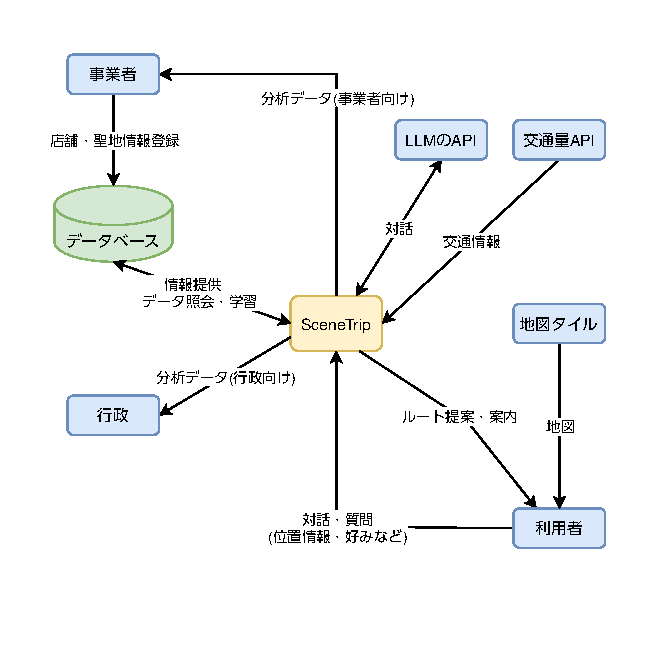
\includegraphics[bb=24.119999 43.253999 266.480711 285.137991,clip]{softinfo.pdf}
	\caption{SceneTripにおける情報の流れ}\label{fig:info}
\end{figure}

\subsection{金銭の流れ}
%--- システムにおける金銭(またはポイント)の流れを図で示す---%
\begin{figure}[H]
	\centering
	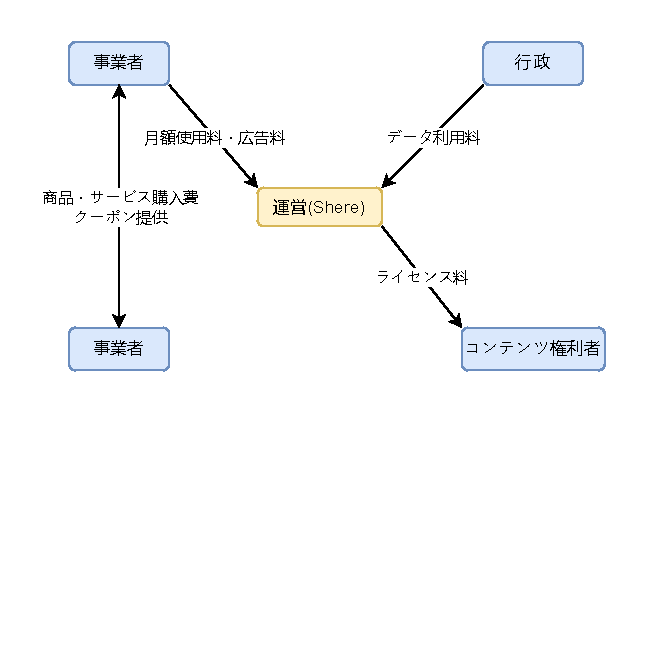
\includegraphics[bb=20.501999 132.281996 291.455991 291.113991,clip]{softmoney.pdf}
	\caption{SceneTripにおける金銭の流れ}\label{fig:money}
\end{figure}


%%%%%%%%%%%%%%%%%%%%%%%%%%%%%%%%%%%%%%%%%%%%%%%%%%%%%%%%%%%%
% 5. 想定する利用者
%%%%%%%%%%%%%%%%%%%%%%%%%%%%%%%%%%%%%%%%%%%%%%%%%%%%%%%%%%%%
\section{想定する利用者}
%--- このシステムの主なターゲットユーザーを箇条書きで記述。---%
\begin{itemize}
	\item 聖地巡礼者
	\item 周遊・体験を重視するアクティブな観光客
	\item デジタルネイティブな情報収集者
\end{itemize}

%%%%%%%%%%%%%%%%%%%%%%%%%%%%%%%%%%%%%%%%%%%%%%%%%%%%%%%%%%%%
% 6. ハードウェア構成・ソフトウェア構成
%%%%%%%%%%%%%%%%%%%%%%%%%%%%%%%%%%%%%%%%%%%%%%%%%%%%%%%%%%%%
\section{ハードウェア構成・ソフトウェア構成}
\subsection{ハードウェア構成}
%--- システムに必要なハードウェア構成を表で示す。---%
\begin{table}[H]
	\centering
	\caption{ハードウェア構成}\label{tab:hardware}
	\begin{tabularx}{0.9\textwidth}{|l|p{9\zw}|X|p{10\zw}|}
		\hline
		\thead{項目} & \thead{種類} & \thead{数量} & \thead{備考} \\ \hline
		メインサーバ & OCI Compute & 1台 & Always Freeサービス(無料枠)\\ \hline
		データベースサーバ & OCI Compute & 1台 & Always Freeサービス(無料枠)\\ \hline
		管理者端末 & PCおよびスマートフォン & 管理者数 & \\ \hline
		利用者端末 & PCおよびスマートフォン & 利用者数 & \\ \hline
	\end{tabularx}
\end{table}

\subsection{ソフトウェア構成}
%--- システムに必要なソフトウェア構成を表で示す。---%
\begin{table}[H]
	\centering
	\caption{ソフトウェア構成}\label{tab:software}
	\begin{tabularx}{0.9\textwidth}{|l|l|X|}
		\hline
		\thead{項目} & \thead{ソフトウェア} & \thead{備考} \\ \hline
		Webサーバ & Nginx & \\ \hline
		データベース & MariaDB & \\ \hline
		バックエンド & PHP(Laravel) & \\ \hline
		フロントエンド & TypeScript & \\ \hline
		端末OS & Android、Linux、Windows、iOS、macOS & \\ \hline
		端末ブラウザ & Firefox、Google Chrome & \\ \hline
		LLM & Google AI Studio & \\ \hline
		地図 & OpenStreetMap & \\ \hline
	\end{tabularx}
\end{table}

%%%%%%%%%%%%%%%%%%%%%%%%%%%%%%%%%%%%%%%%%%%%%%%%%%%%%%%%%%%%
% 7. 運用・保守
%%%%%%%%%%%%%%%%%%%%%%%%%%%%%%%%%%%%%%%%%%%%%%%%%%%%%%%%%%%%
\section{運用・保守}
\subsection{運用}
%--- システムリリース後の日常的な運用業務を箇条書きで記述。---%
\begin{itemize}
	\item 事業者データの登録・管理
	\item システムの稼働監視
	\item 定期的なデータバックアップ
	\item セキュリティ監視
\end{itemize}

\subsection{保守}
%--- システムを正常に維持するための保守業務を箇条書きで記述。---%
\begin{itemize}
	\item インフラのメンテナンス
	\item バグや不具合の調査・修正
	\item OSやミドルウェアのアップデート
\end{itemize}

%%%%%%%%%%%%%%%%%%%%%%%%%%%%%%%%%%%%%%%%%%%%%%%%%%%%%%%%%%%%
% 8. 費用対効果
%%%%%%%%%%%%%%%%%%%%%%%%%%%%%%%%%%%%%%%%%%%%%%%%%%%%%%%%%%%%
\section{費用対効果}
\subsection{効果}
%--- システム導入によって得られる定性的な効果を記述。---%


\subsection{収益}
%--- 5年間など、特定の期間における収益モデルと予測金額を記述。---%
収益は、事業者からの月額利用料、広告収入、行政からの手数料を想定します。
\begin{itemize}
	\item \emph{事業者利用料:} $\text{xxxx円/月}\times\text{xxx事業者}
	\times\text{xxヶ月}=\text{xxxxx円}$
	\item \emph{広告収入:} $\text{xxxx円/月}\times\text{xxヶ月}
	=\text{xxxxx円}$
	\item \emph{手数料収入:} $\cdots$
\end{itemize}
\emph{5年間の総収益: XX,XXX,XXX 円}

\subsection{費用}
%--- 開発にかかる初期費用と、運用にかかる費用を表や数式で示します。---%
\begin{itemize}
	\item \emph{初期費用(開発費):}
		\begin{itemize}
			\item 人件費: $\text{7人日/月}\times\text{7名}\times\text{5ヶ月}
			=\cdots$
			\item その他(機材費など): $\cdots$
		\end{itemize}
		\emph{初期費用合計: XX,XXX,XXX 円}
	\item \emph{運用費用(5年間):}
		\begin{itemize}
			\item サーバ費用: $\text{xxxxx円/月}\times\text{xxヶ月}
			=\text{xxxxx円}$
			\item 維持管理費(人件費など): $\cdots$
		\end{itemize}
		\emph{5年間の運用費用合計: X,XXX,XXX 円}
\end{itemize}
\emph{5年間の総費用: XX,XXX,XXX 円}

\subsection{利益}
%--- 5年間など、特定の期間における利益を計算。---%
5年間で得られる利益は以下の通りです。
$$
\text{総収益} - \text{総費用} = \text{利益}
$$
$$
\text{XX,XXX,XXX円} - \text{XX,XXX,XXX円} = \text{XX,XXX,XXX円}
$$

%%%%%%%%%%%%%%%%%%%%%%%%%%%%%%%%%%%%%%%%%%%%%%%%%%%%%%%%%%%%
% 9. 開発体制と工程計画
%%%%%%%%%%%%%%%%%%%%%%%%%%%%%%%%%%%%%%%%%%%%%%%%%%%%%%%%%%%%
\section{開発体制と工程計画}

%--- 開発チームの体制について記述. ---%
本システムの開発は、高知工科大学情報学群の学生7名からなるグループShareが行います。

%--- 開発スケジュール(ガントチャートなど)を図で示す。---%
また、開発モデルとしてウォーターフォールモデルを採用し、
\cref{fig:gantt}に示す工程で開発します。
\begin{figure}[H]
	\centering
	\begin{ganttchart}[
		canvas/.append style={fill=none,ultra thick},
		title/.append style={fill=none},
		title height=1,
		title label text={\emph{#1}},
		hgrid={draw},
		x unit=16pt,
		y unit chart=34pt,
		bar/.style={},
		bar label node/.append style={font=\normalsize,align=right},
		left label/.style={
			bar/.style={draw,thick,fill=gray!60},
			bar inline label anchor=west,
			bar inline label node/.style={anchor=east},
			inline,
		},
		right label/.style={
			bar inline label anchor=east,
			bar inline label node/.style={anchor=west},
			inline,
		},
	]{0}{20}
		\gantttitle{2025年}{14}
		\gantttitle{2026年}{7}\\
		\gantttitle{9月}{2}
		\gantttitle{10月}{4}
		\gantttitle{11月}{4}
		\gantttitle{12月}{4}
		\gantttitle{1月}{4}
		\gantttitle{2月}{3}\\
		\ganttbar{要求分析}{0}{0}
		\ganttbar[left label]{10/2}{2}{5}
		\ganttbar[right label]{10/30}{2}{5}\\
		\ganttbar{外部設計}{0}{0}
		\ganttbar[left label]{10/30}{6}{9}
		\ganttbar[right label]{12/1}{6}{9}\\
		\ganttbar{内部設計}{0}{0}
		\ganttbar[left label]{12/1}{10}{12}
		\ganttbar[right label]{12/22}{10}{12}\\
		\ganttbar{コーディング\&\\単体テスト}{0}{0}
		\ganttbar[left label]{12/22}{13}{15}
		\ganttbar[right label]{1/15}{13}{15}\\
		\ganttbar{結合・総合テスト}{0}{0}
		\ganttbar[left label]{1/15}{16}{16}
		\ganttbar[right label]{1/22}{16}{16}\\
		\ganttbar{βテスト}{0}{0}
		\ganttbar[left label]{1/22}{17}{18}
		\ganttbar[right label]{2/5}{17}{18}
	\end{ganttchart}
	\caption{工程計画}\label{fig:gantt}
\end{figure}

%%%%%%%%%%%%%%%%%%%%%%%%%%%%%%%%%%%%%%%%%%%%%%%%%%%%%%%%%%%%
% 10. システムのアピールポイント
%%%%%%%%%%%%%%%%%%%%%%%%%%%%%%%%%%%%%%%%%%%%%%%%%%%%%%%%%%%%
\section{システムのアピールポイント}
%--- このシステムの最も強調したい強みや特徴を箇条書きで記述。---%
\begin{enumerate}
	\item \emph{}
	\item \emph{}
	\item \emph{}
	\item \emph{}
\end{enumerate}

%%%%%%%%%%%%%%%%%%%%%%%%%%%%%%%%%%%%%%%%%%%%%%%%%%%%%%%%%%%%
% 参考文献
%%%%%%%%%%%%%%%%%%%%%%%%%%%%%%%%%%%%%%%%%%%%%%%%%%%%%%%%%%%%
\begin{thebibliography}{99}
	%--- 提案書作成にあたり参考にした文献やWebサイトを記述。---%
	\bibitem{ref1}
	著者名, 「文献名」, 出版社, 出版年。

	\bibitem{ref2}
	団体名, “ウェブサイト名”, URL, 閲覧日。
\end{thebibliography}

\end{document}
